\documentclass[12pt,a4paper]{article}
\usepackage[utf8]{inputenc}
\usepackage[german]{babel}
\usepackage[T1]{fontenc}
\usepackage{times}
\usepackage{graphicx}
\usepackage{url}
\usepackage{color}
\usepackage{setspace}
\usepackage{enumerate}
\usepackage{amsmath}
\usepackage{amsfonts}
\usepackage{amssymb}
\usepackage{mathtools}
\usepackage{float}
\usepackage{stix}
\title{Zusammenfassung Quantum Computing}


\newcommand{\ecb}[1]{\{#1\}}
\newcommand{\ket}[1]{\vert #1 \rangle}

\newcommand*\vv[2]{
    \begin{bmatrix}#1\\#2\end{bmatrix}
}

\newcommand*\vvvv[4]{
    \begin{bmatrix}#1\\#2\\#3\\#4\end{bmatrix}
}


\newcommand{\red}[1]{\textcolor{red} {#1}}
\newcommand{\blue}[1]{\textcolor{blue} {#1}}
\newcommand{\green}[1]{\textcolor{Green} {#1}}
\newcommand{\yellow}[1]{\textcolor{yellow} {#1}}
\newcommand{\magenta}[1]{\textcolor{magenta} {#1}}
\newcommand{\cyan}[1]{\textcolor{Aquamarine} {#1}}
\newcommand{\orange}[1]{\textcolor{orange} {#1}}

\author{Henrik Tscherny}
\begin{document}
\maketitle
\tableofcontents

\section{Basic}
\subsection{QBits}
\begin{itemize}
\item \textbf{state of a single QB}: $\ket{s} = a_0 \ket{0} + a_1 \ket{1} = a_0 \vv{1}{0} + a_1 \vv{0}{1} = \vv{a_0}{a_1}$
\item \textbf{state of two QBs}: $\ket{s} = a_0 \ket{00} + a_1 \ket{01} + a_2 \ket{10} + a_3 \ket{11}$
\item \textbf{basis vectors}: $\ket{0} = \vv{1}{0}$,  $\ket{1} = \vv{0}{1}$
\item $P(\ket{0}) = |a_0|^2$, $P(\ket{1}) = |a_1|^2$
\item $\displaystyle \sum_{i=0}^{2^n-1} |a_n| = 1$ (for n-qubit system)
\item \textbf{tensor product}: $\ket{00} = \ket{0} \bigotimes \ket{0} = \vv{1}{0} \bigotimes \vv{1}{0} = \vv{1\vv{1}{0}}{0\vv{1}{0}} = \vvvv{1}{0}{0}{0}$
\item \textbf{entanglement}: non-serperable state (can not be written as the product of qubits, the qubits are statistical dependent)\\
Example: $\ket{\psi} = \frac{1}{\sqrt{2}}\ket{00} + \frac{1}{\sqrt{2}}\ket{11}$
\end{itemize}

\subsection{Complex Numbers}
\begin{itemize}
\item $z = a + ib\\= r \cdot e^{i\varphi}\\= r\cdot (cos \varphi + i \cdot sin \varphi)$\\with $a,b \in \mathbb{R}$ and $i^2 = -1$
\item \textbf{conjugate}: $\bar{z}= a-bi$
\end{itemize}

\subsection{Matrices}
\begin{itemize}
\item \textbf{Transpose}: $A^\top$ swap rows and cols
\item \textbf{Conjugate}: $A^*$ each entry is the conjugate
\item \textbf{Adjunct}: $A^\dagger$ transpose + conjugate
\item \textbf{Unitary}: $UU^\dagger = UU^{-1} = I = U^\dagger U$ adjunct is also the inverse
\item Note: every unitary operator can be written as its eigenbases
\end{itemize}

\section{Gates}
\begin{itemize}
\item every gate is reversible (as gates are unitary matrices)
\item \textbf{Hardamard Gate}:
\begin{itemize}
\item $H = \frac{1}{\sqrt{2}}\ \begin{bmatrix}1 & 1\\1 & -1 \end{bmatrix}$
\item $H \ket{0} = \frac{1}{\sqrt{2}}(\ket{0}+\ket{1})$
\item applying $H$ splits the probabilities in $\frac{1}{2}$ for each (simulate coinflip)
\item $H$ is self inverse as it is unitary
\item \textbf{recursive definition for Hardamard}:\\
$H^{\bigotimes n} = H \bigotimes H^{\bigotimes n-1} = \frac{1}{\sqrt{2}} \begin{bmatrix}1 & 1\\1 & -1 \end{bmatrix} \bigotimes H^{\bigotimes n-1} = \frac{1}{\sqrt{2}} \begin{bmatrix}H^{\bigotimes n-1} & H^{\bigotimes n-1}\\H^{\bigotimes n-1} & -H^{\bigotimes n-1} \end{bmatrix}$\\
$H^{\bigotimes 1} = H$
\end{itemize}
\item \textbf{Pauli Gates}:
\begin{itemize}
\item \textbf{Pauli-X}: Swaps $\ket{0}$ and $\ket{1}$, $X = \begin{bmatrix}0 & 1\\1 & 0 \end{bmatrix}$
\item \textbf{Pauli-Y}: Swaps amplitudes, (adds phase ?), negates amplitudes of $\ket{1}$ $Y = \begin{bmatrix}0 & -i\\i & 0 \end{bmatrix}$
\item \textbf{Pauli-Z}: Negates amplitudes of $\ket{1}$ $Z = \begin{bmatrix}1 & 0\\0 & -1 \end{bmatrix}$
\end{itemize}

\item \textbf{CNot}:
\begin{itemize}
\item negates the target if the controller is active
\item permutation matrix
\item $CNOT = \begin{bmatrix}1 & 0 & 0 & 0\\0 & 1 & 0 & 0\\0 & 0 & 0 & 1\\0 & 0 & 1 & 0 \end{bmatrix}$
\end{itemize} 
\end{itemize}

\subsection{Phase Kickback}
\begin{itemize}
\item U: one qubit unitary gate 
\item $\ket{\phi}$: some base state 
\item applying $U$ to $\ket{\psi}$ yields $e^{i\phi}\ket{\psi}$
\item the global phase factor of a quantum state is not measurable (symmetry)
\item using \textbf{ancilla} qubits the global phase can be turned intro a relative phase which is measurable
\end{itemize}

\section{Deutsch Algorithm}
\begin{itemize}
\item function $f : \ecb{0,1}\rightarrow \ecb{0,1}$ that is either balanced or constant
\item classical: compute f on every input
\item quantum: one call of f is needed
\item quantum oracle:
\begin{itemize}
\item $U_f : \ket{x}\ket{y} \xrightarrow{U_f} \ket{x}\ket{y\bigoplus f(x)}$
\item $\ket{x}$ input to function
\item $\ket{y}$ qubit to write function result to
\item $\ket{y\bigoplus f(x)}$, the XOR ensures that the oracle is reversible (as each image has a unique preimage)
\item initializing $y = \ket{0}$ we only get the function value $\ket{x}\ket{f(x)}$ as $0\bigoplus x = x$
\item initializing $y = \ket{-}$ we get phase kickback to $\ket{x}\ket{-} \xrightarrow{U_f} (-1)^{f(x)} \ket{x}\ket{-}$ (a phase is applied to the input qubit)\\$\begin{cases} \ket{x}\ket{-} & f(x)=0 \\ -\ket{x}\ket{-} & f(x)=1 \end{cases}$
\item Note: this is called a phase oracle ($U_f \ket{x}\ket{-} = (-1)^{f(x)}\ket{x}\ket{-}$)
\end{itemize}
\item 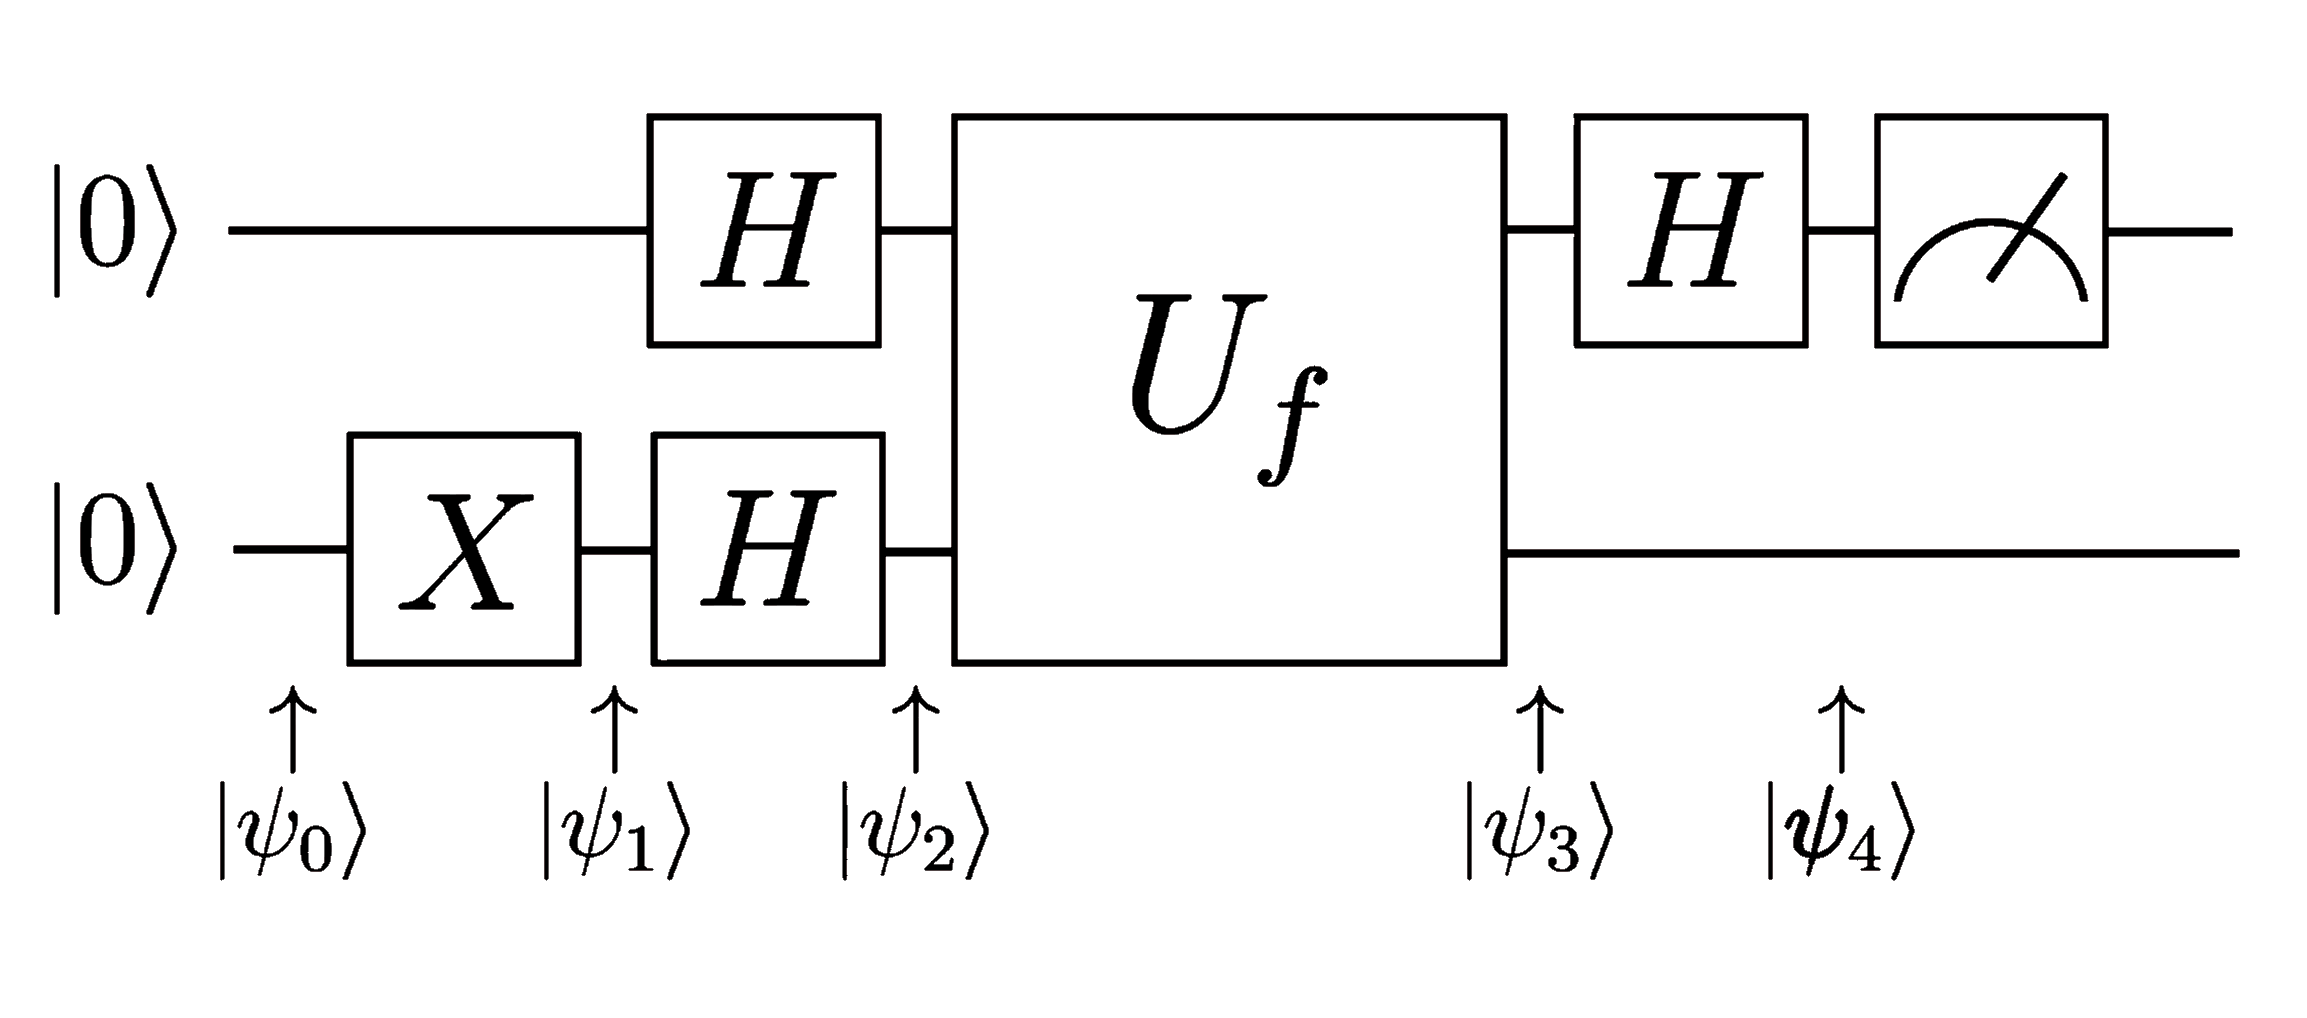
\includegraphics[scale=0.2]{./resources/deutschplan.png}
\begin{itemize}
\item $\ket{\psi_0} = \ket{00}$
\item $\ket{\psi_1} = \ket{01}$
\item $\ket{\psi_2} = \ket{+-} = \frac{1}{\sqrt{2}}(\ket{0} + \ket{1})\ket{-} = \frac{1}{\sqrt{2}}(\ket{0}\ket{-}+\ket{1}\ket{-})$
\item $\ket{\psi_3} = U_f \frac{1}{\sqrt{2}}(\ket{0}\ket{-}+\ket{1}\ket{-}) = \frac{1}{\sqrt{2}}(U_f\ket{0}\ket{-}+U_f\ket{1}\ket{-}) \overset{\text{phase oracle}}{=} \frac{1}{\sqrt{2}}((-1)^{f(0)}\ket{0}\ket{-}+ (-1)^{f(1)}\ket{1}\ket{-})$\\($\ket{-}$ can be omitted as its not needed)
\item case $f(0) = f(1)$: $\begin{cases} \ket{\psi_3} = \frac{1}{\sqrt{2}}(\ket{0} + \ket{1}), & f(0) = f(1) = 0\\ \ket{\psi_3} = -\frac{1}{\sqrt{2}}(\ket{0}+\ket{1}), & f(0) = f(1) = 1 \end{cases}$\\$\ket{\psi_3} = \pm \frac{1}{\sqrt{2}}(\ket{0}+\ket{1}) = \pm \ket{+}$
\item case $f(0) \neq f(1)$: $\begin{cases} \ket{\psi_3} = \frac{1}{\sqrt{2}}(\ket{0} - \ket{1}), & f(0) = 0 \land f(1) = 1\\\ket{\psi_3} = -\frac{1}{\sqrt{2}}(\ket{0} - \ket{1}), & f(0) = 1 \land f(1) = 0 \end{cases}$\\$\ket{\psi_3} = \pm \frac{1}{\sqrt{2}}(\ket{0}-\ket{1}) = \pm \ket{-}$
\item $\ket{\psi_4} = \begin{cases} \pm \ket{0}, & f(0) = f(1)\\ \pm\ \ket{1}, & f(0) \neq f(1) \end{cases}$
\end{itemize}
\item measuring 0 iff function is constant and 1 iff function is balanced
\end{itemize}

\section{Deutsch-Jozsa Algorithm}
\begin{itemize}
\item generalized version of Deutsch Algorithm to n qubits
\item $f : \ecb{0,1}^n \rightarrow \ecb{0,1}$
\item f is constant iff $\forall x, f(x) = c$
\item f is balanced iff $|\ecb{x \mid f(x) = 0}| = |\ecb{x \mid f(x) = 1}|$
\item classical: $2^{n-1}+1$ function calls (input half the possible inputs)
\item quantum: one call of f in needed (exponential speed up)
\item 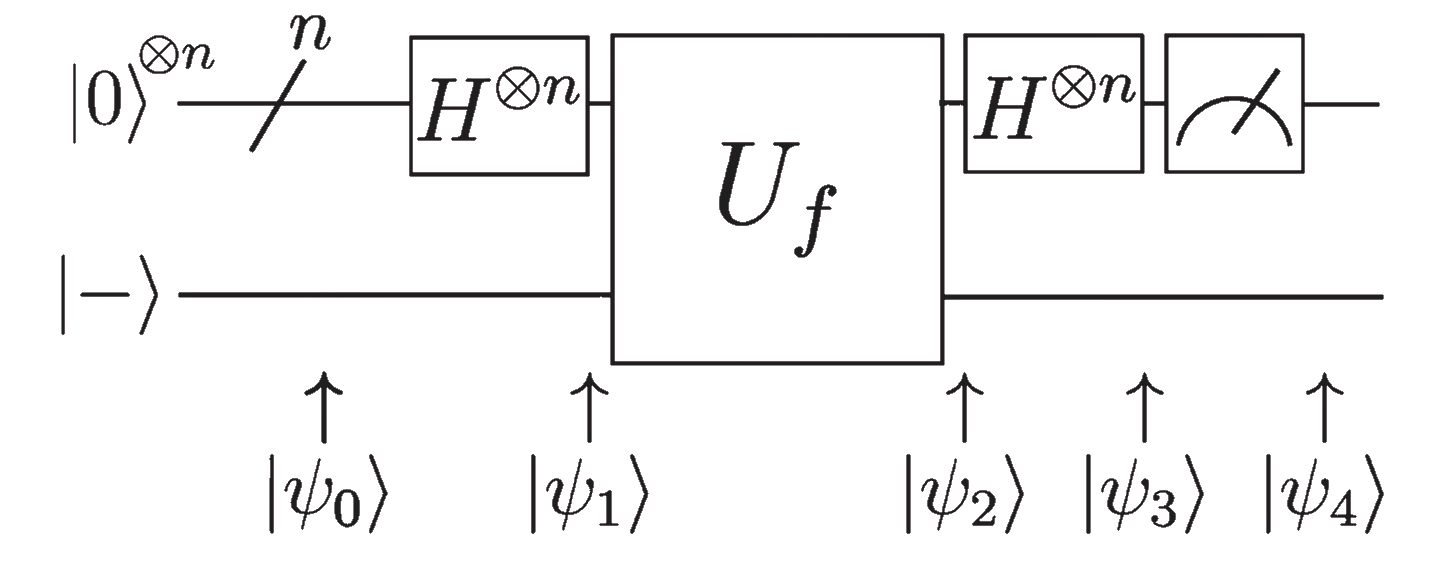
\includegraphics[scale=0.3]{./resources/jozsaplan.png}
\begin{itemize}
\item $\ket{\psi_0} = \ket{00...0}\ket{-} = \ket{0}^{\bigotimes n}\ket{-}$ (we can get the $\ket{-}$ by $H\ket{1}$)
\item $\displaystyle \ket{\psi_1} = H^{\bigotimes n}\ket{0}^{\bigotimes n}\ket{-} = \frac{1}{\sqrt{2^n}} \sum_{x\in\ecb{0,1}^n} \ket{x}\ket{-}$ (uniform distribution)
\item $\displaystyle \ket{\psi_2} = \frac{1}{\sqrt{2^n}} \sum_{x\in\ecb{0,1}^n}U_f\ket{x}\ket{-} \overset{\text{phase oracle}}{=} \frac{1}{\sqrt{2^n}} \sum_{x\in\ecb{0,1}^n} (-1)^{f(x)}\ket{x}\ket{-}$\\($\ket{-}$ can be omitted)
\item Note: $\displaystyle H^{\bigotimes n}\ket{x} = \frac{1}{\sqrt{2^n}} \sum_{z\in\ecb{0,1}^n} (-1)^{x\cdot z} \ket{z}$, $\; (\ast)$
\item $\displaystyle \ket{\psi_3} = \frac{1}{\sqrt{2^n}} \sum_{x\in\ecb{0,1}^n} (-1)^{f(x)}H^{\bigotimes n}\ket{x}\ket{-}\\\overset{(\ast)}{=}
\frac{1}{\sqrt{2^n}} \sum_{x\in\ecb{0,1}^n} (-1)^{f(x)}\frac{1}{\sqrt{2^n}} \sum_{z\in\ecb{0,1}^n} (-1)^{x\cdot z} \ket{z}\\= \frac{1}{2^n}\sum_{x\in\ecb{0,1}^n}\sum_{z\in\ecb{0,1}^n} (-1)^{f(x)+x\cdot z} \ket{z}$
\item consider the amplitude of $\ket{0}^{\bigotimes n}$ is $\displaystyle \frac{1}{2^n} \sum_{x\in\ecb{0,1}^n} (-1)^{f(x)}$
case f constant: $\displaystyle \begin{cases} \frac{1}{2^n} \sum_{x\in\ecb{0,1}^n} (-1)^0 = \frac{1}{2^n} 2^n = 1, & f(x) = 0\\\frac{1}{2^n} \sum_{x\in\ecb{0,1}^n} (-1)^1 = \frac{1}{2^n} (-2^n) = -1, & f(x)=1 \end{cases}$
\item hence if f is constant the probability of measuring all zeros is 1
\item hence if f is balanced half of the sum is 1 and half is -1 hence the probability of measuring all zeros is 0
\item $\rightarrow$ measure and iff we get 000...0 then $f(x)$ is constant else balanced
\end{itemize}
\end{itemize}

\section{Grovers Algorithm}
\begin{itemize}
\item Problem: given an unstructured database, find an element $\hat{x}$ within this database
\item $f : \ecb{0,1}^n \rightarrow \ecb{0,1}$ with $f(\hat{x}) = 1$, $f(\lnot \hat{x}) = 0$ \hspace{1cm}($x, \hat{x} \in \ecb{0,1}^n$)
\item classical: $\frac{N+1}{2} \in O(N)$
\item quantum: $\frac{\pi}{4}\sqrt{N} \in O(\sqrt{N})$
\item Steps:
\begin{enumerate}
\item generate uniform distribution on all elements:\\
\begin{itemize}
\item $\displaystyle H^{\bigotimes n}\ket{000...0}=\frac{1}{\sqrt{N}} \sum_{x=0}^{N-1} \ket{x}$
\item $\displaystyle\ket{s} = H^{\bigotimes n+1} \ket{000...0}\ket{1} = \ket{0}^{\bigotimes n}\ket{-}$
\end{itemize}
\item Grover Iteration:
\begin{enumerate}
\item Negate the amplitude of $\hat{x}$ (Oracle $\hat{U_f}$)
\begin{itemize}
\item $\displaystyle \hat{U_f}\ket{s} = \frac{1}{\sqrt{2^n}} \sum_{x\in\ecb{0,1}^n} (-1)^{f(x)}H^{\bigotimes n}\ket{x}\ket{-}$ \hspace{0.2cm}(as in Deutsch-Josza)
\end{itemize}
\item Mirror/Reflect/Diffuse all amplitudes a at the mean value m(Diffusion $\hat{D}$)
\begin{itemize}
\item $a := 2\cdot m - a$
\item mirroring as a quantum state: $\displaystyle \sum_{i=0}^{N-1} a_i \ket{i}$ $(\ast)$
\item mean value of amplitudes: $\displaystyle \sum_{j=0}^{N-1} \frac{a_j}{N}$ $(\ast\ast)$
\item combining $(\ast)$ and $(\ast\ast)$ we get: $\displaystyle\ket{s} = \sum_{i=0}^{N-1} \bigg( 2\cdot \sum_{j=0}^{N-1} \frac{a_j}{N}\bigg) \ket{i}$
\item $D_N = \begin{bmatrix} -1 + \frac{2}{N} & \dots & \frac{2}{N} \\ \vdots & -1 + \frac{2}{N}& \vdots\\  \frac{2}{N} & \dots & -1 + \frac{2}{N}\end{bmatrix}$
\item Note: $D_N$ can be expressed as a local operation ($leq 3$ bits involved)
\end{itemize}
\end{enumerate}
\item Conditional sign flip for $\hat{x}$
\begin{itemize}
\item $V_f : \ket{x} \rightarrow (-1)^{f(x)}\ket{x}$
\end{itemize}
\item Measure $\ket{x}$ and return it off $\hat{x}>c$ (c is some constant)
\end{enumerate}
\item The number of grover iterations T is capped by $(2T+1)\frac{1}{\sqrt{N}}$ since every iteration rotates by $\frac{2}{\sqrt{N}}$ $\Rightarrow$ $T=\frac{\pi}{4}\sqrt{4}$
\item doing more than the necessary number of iteration degrades the result
\end{itemize}

\section{Simons Algorithms}
Todo

\section{Shors Algorithm}
Todo

\end{document}